\newpage
\section{Экспериментальная часть}

Проведем тестирование и сравним алгоритмы по времени работы.

\subsection{Примеры работ}

Ниже приведены примеры работ при корректных и некорректных данных

\begin{figure}[H]
    \centering
    
\includegraphics[scale=0.5]{zero_arg}
    \caption{Без аргументов}
    \label{img:zero-arg}
\end{figure}

\begin{figure}[H]
    \centering
    
\includegraphics[scale=0.5]{less_arg}
    \caption{Некорректный один аргумент}
    \label{img:less-arg}
\end{figure}

\begin{figure}[H]
    \centering
    
\includegraphics[scale=0.5]{less_four_arg}
    \caption{Некорректные четыре агрумента}
    \label{img:less-four-arg}
\end{figure}

\begin{figure}[H]
    \centering
    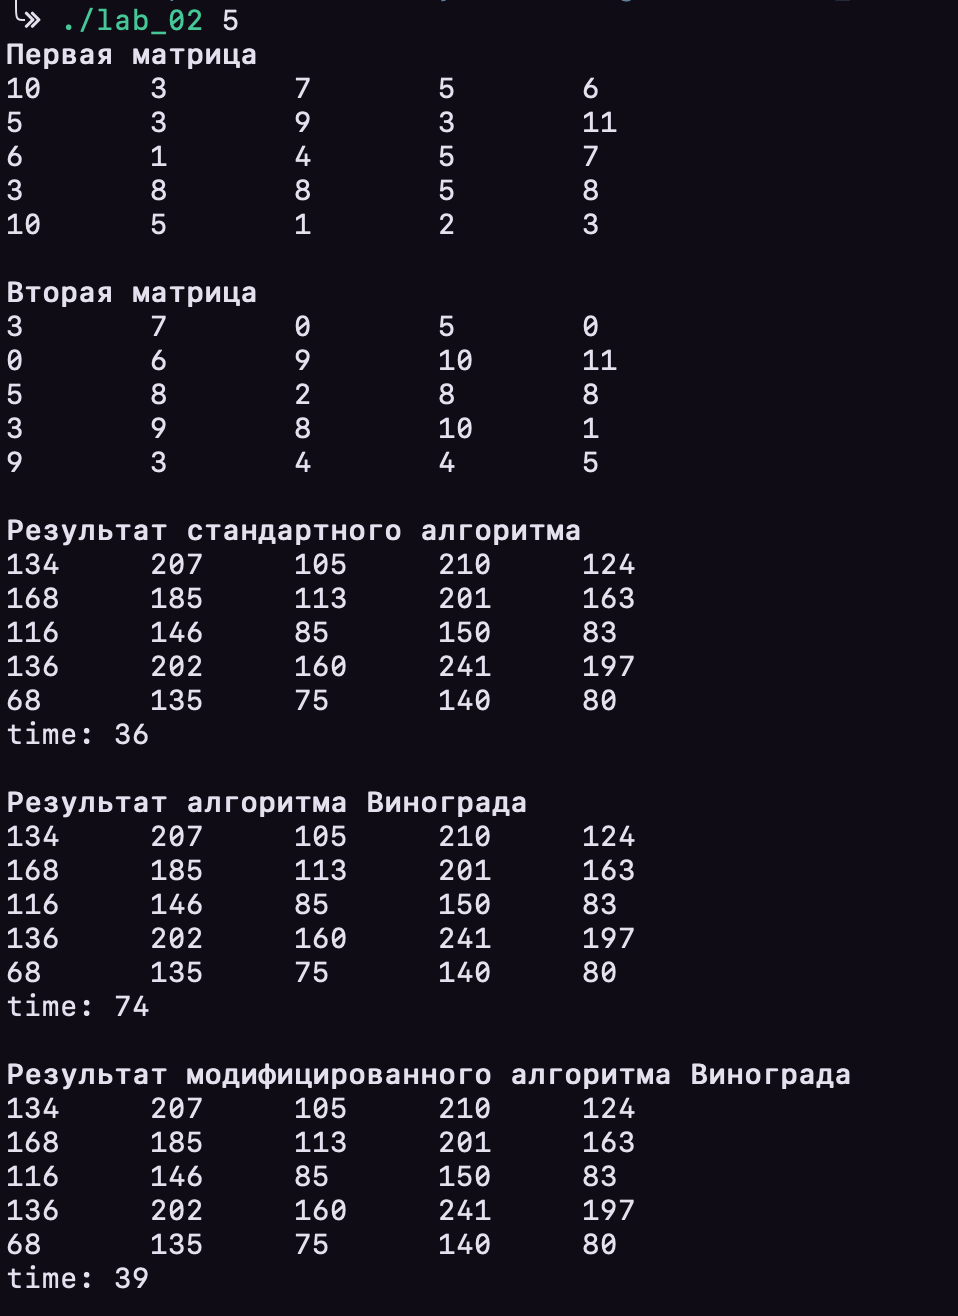
\includegraphics[scale=0.5]{one_arg}
    \caption{Один аргумент}
    \label{img:one-arg}
\end{figure}

\begin{figure}[H]
    \centering
    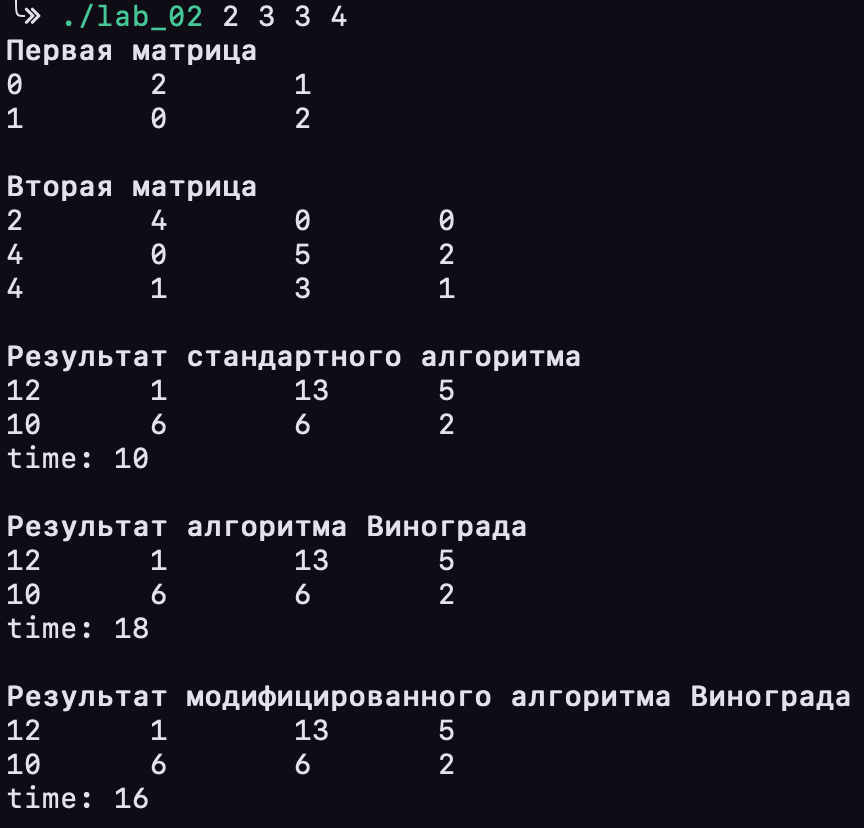
\includegraphics[scale=0.5]{four_arg}
    \caption{Четыре аргумента}
    \label{img:four-arg}
\end{figure}

\subsection{Результаты тестирования}

Для тестирования были использованы тесты из таблицы \ref{table:test}.
Результаты продемонстрированы на таблицах \ref{table:test-default},
\ref{table:test-vin}, \ref{table:test-modvin}.

\begin{table}[H]
    \caption{Результаты стандартного алгоритма}
    \label{table:test-default}
    \centering
    \begin{tabular}{|c|c|c|}
        \hline
        Первая матрца & Вторая матрица & Результат \\
        \hline
        1 2 & 1 2 & \ 7 10 \\
        3 4 & 3 4 & 15 22 \\
        \hline
        1 2 3 & 1 2 3 & \ 30\ \ 36\ \ 42 \\
        4 5 6 & 4 5 6 & \ 66\ \ 81\ \ 96 \\
        7 8 9 & 7 8 9 & 102 126 150 \\
        \hline
        1 2 3 & 1 & 14 \\
        4 5 6 & 2 & 32 \\
              & 3 & \\
        \hline
    \end{tabular}
\end{table}

\begin{table}[H]
    \caption{Результаты алгоримта Винограда}
    \label{table:test-vin}
    \centering
    \begin{tabular}{|c|c|c|}
        \hline
        Первая матрца & Вторая матрица & Результат \\
        \hline
        1 2 & 1 2 & \ 7 10 \\
        3 4 & 3 4 & 15 22 \\
        \hline
        1 2 3 & 1 2 3 & \ 30\ \ 36\ \ 42 \\
        4 5 6 & 4 5 6 & \ 66\ \ 81\ \ 96 \\
        7 8 9 & 7 8 9 & 102 126 150 \\
        \hline
        1 2 3 & 1 & 14 \\
        4 5 6 & 2 & 32 \\
              & 3 & \\
        \hline
    \end{tabular}
\end{table}

\begin{table}[H]
    \caption{Результаты оптимизированного алгоритма Винограда}
    \label{table:test-modvin}
    \centering
    \begin{tabular}{|c|c|c|}
        \hline
        Первая матрца & Вторая матрица & Результат \\
        \hline
        1 2 & 1 2 & \ 7 10 \\
        3 4 & 3 4 & 15 22 \\
        \hline
        1 2 3 & 1 2 3 & \ 30\ \ 36\ \ 42 \\
        4 5 6 & 4 5 6 & \ 66\ \ 81\ \ 96 \\
        7 8 9 & 7 8 9 & 102 126 150 \\
        \hline
        1 2 3 & 1 & 14 \\
        4 5 6 & 2 & 32 \\
              & 3 & \\
        \hline
    \end{tabular}
\end{table}

Все тесты пройдены успешно.

\subsection{Замеры времени}

На рисунке \ref{img:even} представлены результаты замера времени алгоритмов при
четных размерностях, а на рисунке \ref{img:noteven} при нечетных размерностях матриц.
Оба случая прогонялись на квардатных матрицах.

\begin{figure}[H]
    \begin{tikzpicture}
        \begin{axis}[
            legend pos = north west,
            xlabel=Размерность матрицы,
            ylabel=микросекунды,
            grid = major,
            width = 0.8\paperwidth,
            height = 0.38\paperheight,
            line width = 1
        ]
            \legend{
                Обычный алгоритм,
                Алгоритм Винограда,
                Оптимизированный алгоритм Винограда
            };
            \addplot[dashed] coordinates {
                (100, 34501)
                (200, 273438)
                (300, 911536)
                (400, 2287721)
                (500, 4467987)
                (600, 7982696)
                (700, 12589205)
                (800, 19543501)
                (900, 29907202)
                (1000, 39608083)
            };

            \addplot[black] coordinates {
                (100, 18468)
                (200, 141549)
                (300, 509012)
                (400, 1465966)
                (500, 2716895)
                (600, 4893372)
                (700, 7788205)
                (800, 11974361)
                (900, 17429652)
                (1000, 24443640)
            };

            \addplot[dotted] coordinates {
                (100, 15781)
                (200, 117581)
                (300, 438752)
                (400, 1146582)
                (500, 2466496)
                (600, 4238264)
                (700, 6635427)
                (800, 10541381)
                (900, 15063388)
                (1000, 21113694)
            };
        \end{axis}
    \end{tikzpicture}
    \caption{Четная размерность}
    \label{img:even}
\end{figure}

\begin{figure}[H]
    \begin{tikzpicture}
        \begin{axis}[
            legend pos = north west,
            xlabel=Размерность матрицы,
            ylabel=микросекунды,
            grid = major,
            width = 0.8\paperwidth,
            height = 0.38\paperheight,
            line width = 1
        ]
            \legend{
                Обычный алгоритм,
                Алгоритм Винограда,
                Оптимизированный алгоритм Винограда
            };
            \addplot[dashed] coordinates {
                (101, 34170)
                (201, 263159)
                (301, 909942)
                (401, 2262964)
                (501, 4486670)
                (601, 7851527)
                (701, 12517730)
                (801, 19429387)
                (901, 38556411)
                (1001, 62124826)
            };
            \addplot[black] coordinates {
                (101, 19163)
                (201, 142118)
                (301, 544590)
                (401, 1417500)
                (501, 2850727)
                (601, 4809657)
                (701, 7629622)
                (801, 12085389)
                (901, 17761017)
                (1001, 24574933)
            };
            \addplot[dotted] coordinates {
                (101, 15982)
                (201, 119376)
                (301, 442958)
                (401, 1257460)
                (501, 2437730)
                (601, 4266685)
                (701, 6876743)
                (801, 10731128)
                (901, 15011152)
                (1001, 23672051)
            };
        \end{axis}
    \end{tikzpicture}
    \caption{Нечетная размерность}
    \label{img:noteven}
\end{figure}

\subsection{Выводы}

Из графиков зависимости размерности матрицы ко времени ее вычисления
видно, что стандартный алгоритм работает медленне, чем алгоритм
Винограда на 50\%. Также, можно заметить, что оптимизация прошла
успешно и оптимизированный алгоритм Винограда работает быстрее
обычного на 5\%.
